\documentclass{article}

\usepackage{url} 

\usepackage{pdfpages}
\usepackage{lastpage}
\usepackage{fancyhdr}
\usepackage{ngerman}
\usepackage{listings}

\usepackage{tabularx}
\usepackage{floatrow}
\usepackage[tableposition=top]{caption}
\floatsetup[table]{capposition=top}

\usepackage{amsmath, amssymb}

\usepackage[utf8]{inputenc}


\usepackage[numbib]{tocbibind}



\newcommand\twodigits[1]{%
   \ifnum#1<10 0#1\else #1\fi
}



\lhead{Interferometer}
\rhead{13. November 2020\\T. Maier, J. Winkler}
%\cfoot{\twodigits{\thepage}~/ \pageref{LastPage}}
\cfoot{{\thepage}~/ \pageref{LastPage}}

\newcommand{\W}{\text{W}}
\newcommand{\V}{\text{V}}
\newcommand{\A}{\text{A}}


\newcommand{\mini}{\operatorname{min}}


\begin{document}

\parindent0cm

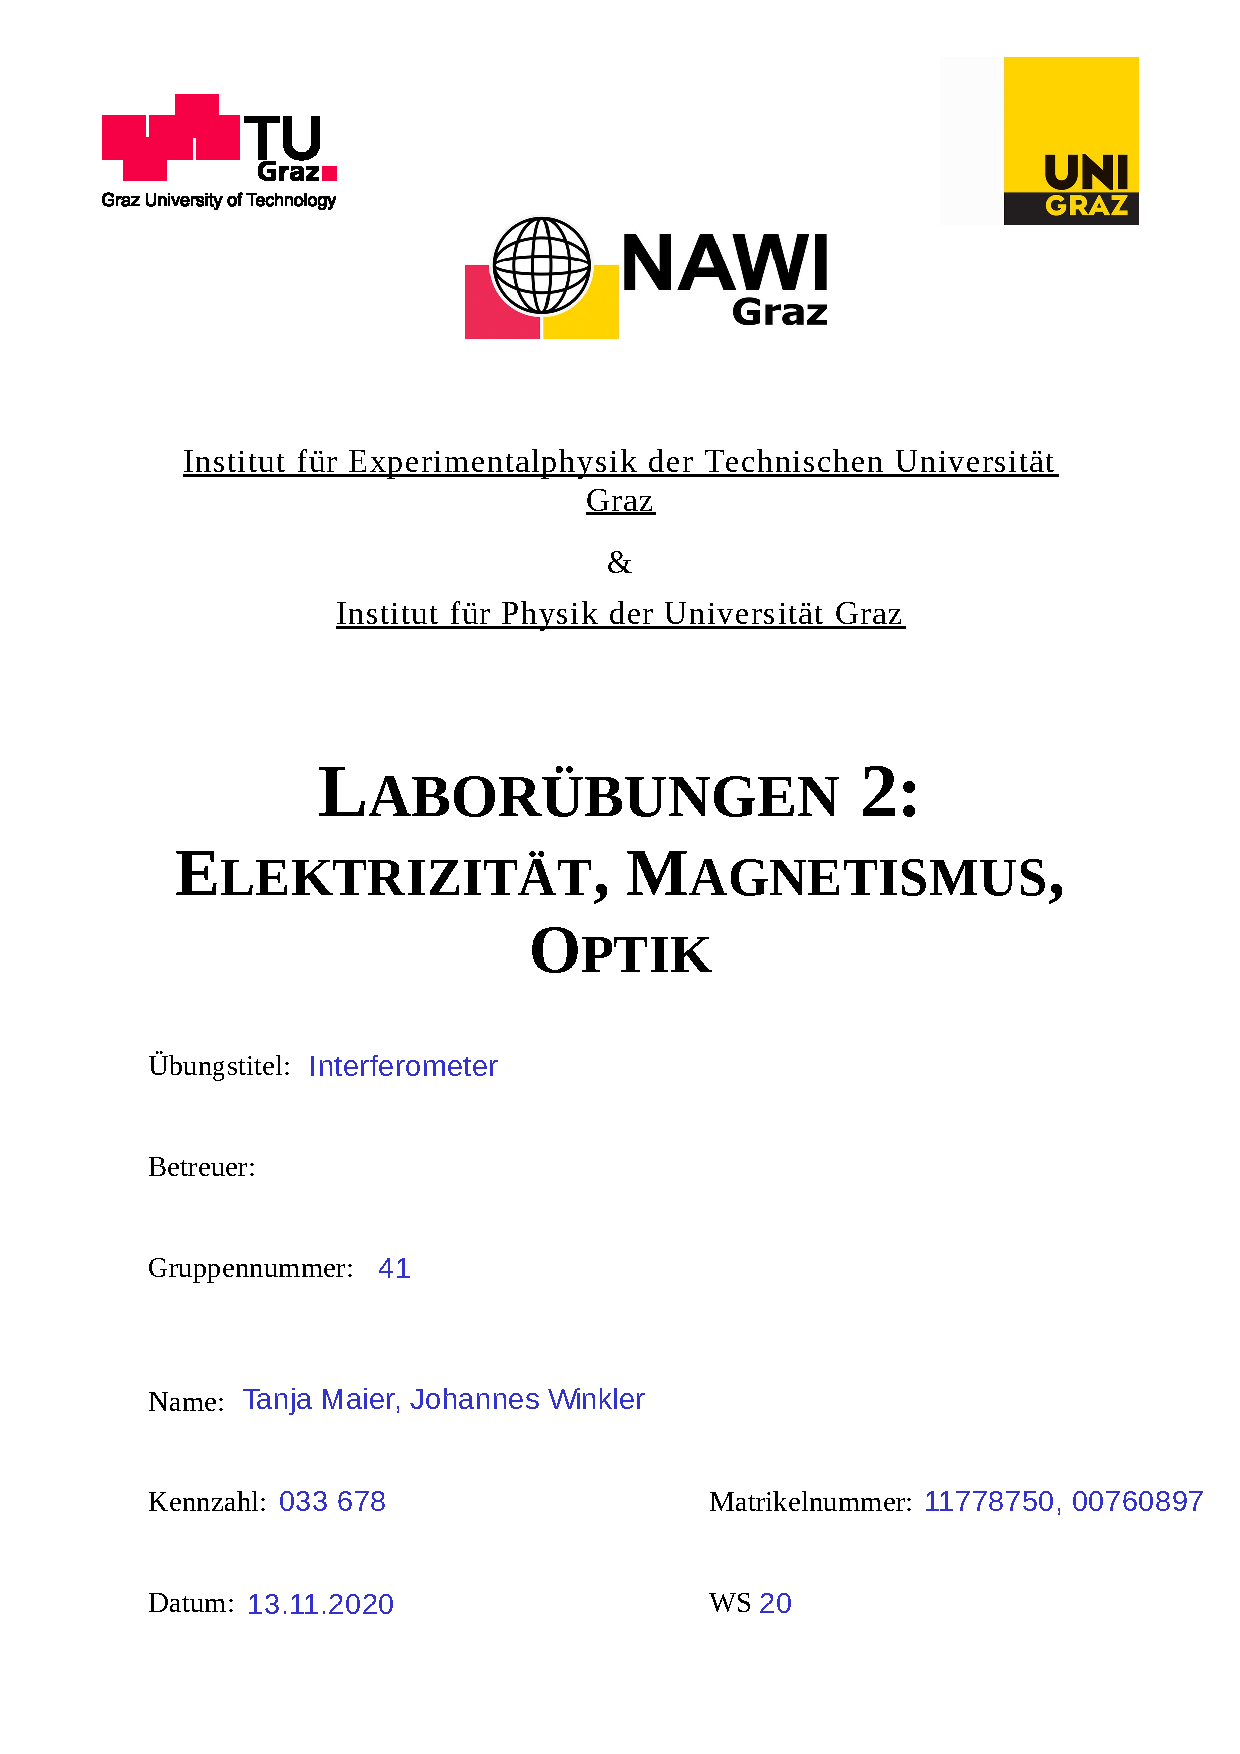
\includepdf{Deckblatt.pdf}


\pagestyle{fancy}

\tableofcontents
\newpage
\section{Aufgabenstellung}

\begin{enumerate}
\item Demonstration und Erklärung des Einflusses der Größe einer Lichtquelle auf das Interferenzmuster eines Doppelspaltes.
\item Demonstration und Erklärung des Einflusses der spektralen Breite des Lichtes einer räumlich kohärenten Lichtquelle auf das Interferenzmuster eines Doppelspaltes.
\item Bestimmung der Dicke einer Kunststoffschicht mit dem Doppelspalt Interferenzmuster.
\item Bestimmung der Größe der Lichtquelle, bei der für Doppelspalten mit unterschiedlichem Spaltabstand das Licht noch räumlich kohärent ist.
\end{enumerate}



\section{Voraussetzungen und Grundlagen}

Grundlage dieses Versuchs bietet die Wellennatur des Lichts. Licht kann als elektromagnetische Welle im sichtbaren Spektralbereich gesehen werden. Das von einer Quelle ausgesendete Licht kann dann mit einem Doppelspalt in mehrere Teilwellen aufgespalten werden. Wenn dieses Teilwellen dann wieder aufeinandertreffen (z.B. durch Totalreflexion an einem Spiegel), so kommt es je nach Gang- bzw. Zeitunterschied entweder zur Auslöschung (destruktive Interferenz) oder Verstärkung (konstruktive Interferenz) der wieder vereinigten Welle. Wichtig ist dabei, dass die Welle sowohl zeitlich als auch räumlich kohärent (Amplitude und Phase sind also an jedem Punkt und zu jeder Zeit eindeutig definiert) ist. Dann gilt
\begin{align}
\Delta s = d \cdot \sin \theta_n = n\cdot \lambda \qquad n\in \mathbb{N}_0
\end{align}
wobei der Gangunterschied der beiden Teilwellen $n$-ter Ordnung, $d$ der Abstand der Spalten, $\theta_n$ der $n$-te Beugungswinkel, n die Ordnung des Interferenzmaximums und $\lambda$ die Wellenlänge ist.

Die Interferenzmaxima werden außerdem mit einer Sammellinse erfasst und abgebildet. Für den Abstand $b_n$ zwischen $0$-tem und $n$-tem Maximum gilt folgender Zusammenhang 
\begin{align}
b_n = f_2 \cdot \tan\left( \operatorname{arcsin}\left(\frac{n\cdot\lambda}{d}\right)\right), \qquad n\in\mathbb{N}_0
\end{align}
wobei $f_2$ die Brennweite der Sammellinse nach dem Doppelspalt ist. Außerdem kann man noch den Kontrast $K$ des Inferenzmusters bestimmen, welcher von der jeweiligen Intensität der Lichtquelle abhängt.
\begin{align}
K = \frac{I_\text{0,max}-I_\text{1,min}}{I_\text{0,max}+I_\text{1,min}} = \left| \frac{\sin\left(\frac{\pi\cdot d\cdot 2\cdot w}{\lambda\cdot f_1}\right)}{ \frac{\pi\cdot d\cdot 2\cdot w}{\lambda\cdot f_1} }\right|
 \label{eq:kontrast}
\end{align}
wobei $I$ die Intensität, $f_1$ die Brennweite der Sammellinse vor dem Doppelspalt und $w$ der Durchmesser der Spaltblende ist (wird als \textit{Größe} der Lichtquelle gesehen). Außerdem wird bei diesem Experiment auch eine Probe mit Polyacrylat verwendet, welche eine zusätzliche Phasenverschiebung am Doppelspalt bewirkt. Diese Phasenverschiebung kann beschrieben werden durch
\begin{align}
\Delta s_0 = \Delta s + t\cdot (n_1-n_2) = d\cdot\sin(\theta)\cdot t\cdot (n_1-n_2)
\end{align}
wobei $t$ die Dicke der Probe, $n_1$ der Brechungsindex der Probe und $n_2$ der Brechungsindex der Umgebung (hier: Luft, also $n_2 = 1$) ist. Durch Umformung ergibt sich
\begin{align}
\label{eq:schichtdicke}
t = \frac{d\cdot \sin(\theta)}{n_1-1}
\end{align}


Zusätzlich wird noch der Umrechnungsfaktor zwischen Pixel und $\mu$m benötigt. Dieser ergibt sich aus der elementaren geometrischen Überlegung, dass eine Distanz $b$ im Interferenzmuster trigonometrisch in folgender Beziehung dargestellt werden kann
\begin{align}
\label{eq:theta}
\tan(\theta) = \frac{b}{f}
\end{align}
wobei $f$ die Brennweite ist. Weil zusätzlich $d\cdot \sin(\theta) = m\cdot \lambda$ gilt, folgt insgesamt
\begin{align*}
b = f\cdot \tan\left(\operatorname{arcsin}\left(\frac{m\cdot \lambda}{d}\right)\right)
\end{align*}
Wenn $f$ in $\mu$m angegeben wird, dann ist auch $b$ in $\mu$m. Man kann entsprechende Distanz zwischen $0$-ten und $m$-ten Maximum auch in Pixel messen. Division ergibt das Verhältnis
\begin{align}
\label{eq:umrechnung}
Z = \frac{b}{|x_0-x_m|} = \frac{f\cdot \tan\left(\operatorname{arcsin}\left(\frac{m\cdot \lambda}{d}\right)\right)}{|x_0-x_m|}
\end{align}



%\begin{figure}[H]
%\caption{Transformator}
%\label{fig:transformator}
%{\centering
%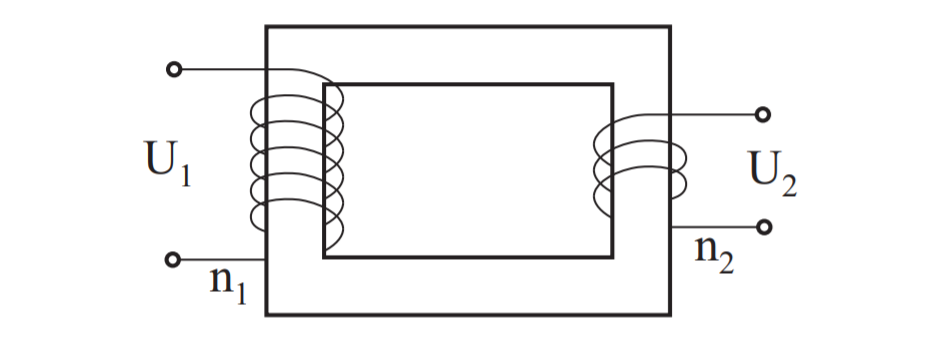
\includegraphics[scale=0.4]{transformator.png}
%~
%}
%\end{figure}





\section{Geräteliste}

\begin{table}[H]
\caption{Liste der verwendeten Geräte}

~

\begin{tabular}{l|p{3cm}p{3cm}llll}
Abk. & Bezeichnung  & Typ & Gerätenummer & Unsicherheit \\
\hline
S & Spaltblende \\
\hline
L1 & Sammellinse 1 & $f_1 = 300~$mm & & $\Delta f_1 = 0.5~$mm \\
\hline
L2 & Sammellinse 2 & $f_2 = 150~$mm & & $\Delta f_2 = 0.5~$mm \\
\hline
L3 & Sammellinse 3 & $f_3 = 40~$mm & & $\Delta f_3 = 0.5~$mm \\
\hline
L4 & Sammellinse 4 & $f_4 = 30~$mm & & $\Delta f_4 = 0.5~$mm \\
\hline
DS1 & Doppelspalt & $d_1=0.43~$mm  & & $\Delta d_1 = 0.005~$mm \\
\hline
DS2 & Doppelspalt & $d_2=0.23$~mm  & & $\Delta d_2 = 0.005~$mm\\
\hline
DS3 & Doppelspalt & $d_3=0.13$~mm & & $\Delta d_3 = 0.005~$mm\\
\hline





B & Lochblenden und Irisblende & $d_1=2~$mm ~ ~ ~ ~ $d_2=3~$mm   ~~~~~~~~~~~~ $d_3=6~$mm & &  $\Delta d = 0.1~$mm \\
\hline
F & Filterrad für LEDs & \\
\hline
K & Kamera
\end{tabular}

\end{table}


\newpage

\section{Beschreibung der Versuchsanordnung}

Der Versuchsaufbau ist maßstabsgetreu in Grafik \ref{fig:aufbau} dargestellt.
\begin{figure}[H]
\caption{Versuchsaufbau. $L_1,L_2,L_3,L_4$ Linsen, $S$ Spaltblende, $DS$ Doppelspalt, $F$ Filterrad, $O$ Substrat mit Polyacrylat-Schicht, $K$ Kamera. Als Maßstab ist 1 Quadrat gleich 20~mm.}
\label{fig:aufbau}
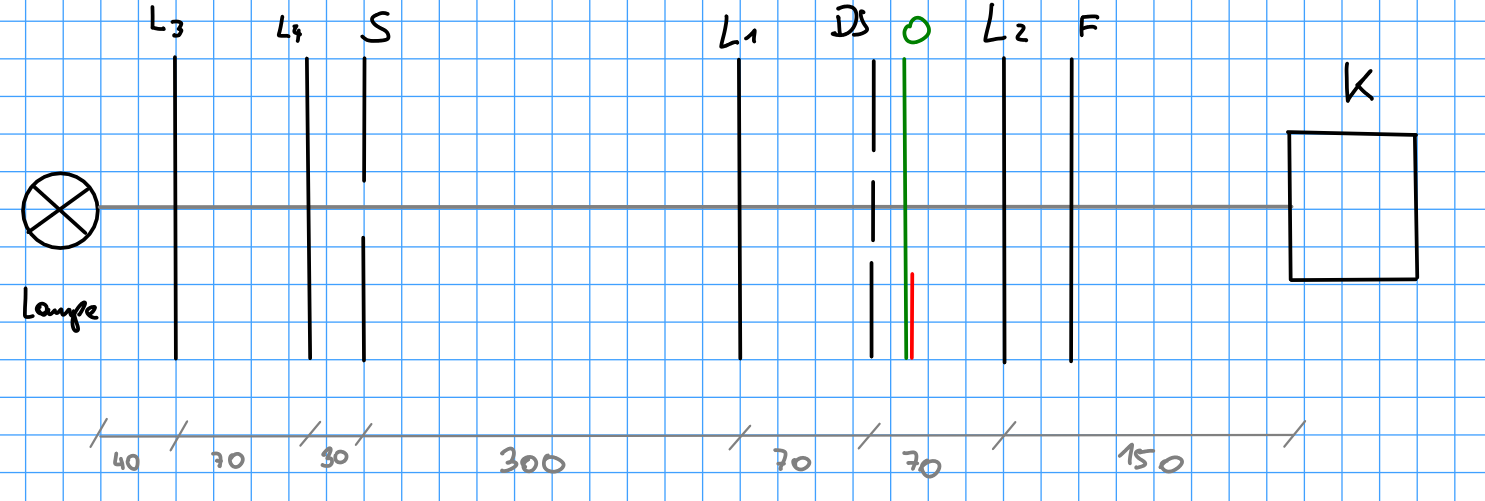
\includegraphics[scale=1]{aufbau.png}
\end{figure}


Die von der Lampe ausgehenden Lichtstrahlen werden in $L_3$ parallelisiert, da der Abstand zur Lampe genau die Brennweite von $L_3$ ist. In $L_4$ wird der Strahl auf den Spalt fokussiert. Die einstellbare Spaltblende liegt exakt im Brennpunkt von $L_1$ und $L_4$, daher werden die ausgehenden Strahlen in $L_1$ wieder parallelisiert. Danach trifft das Licht auf den Doppelspalt, wo Beugung stattfindet. Danach dringt das Licht durch das Substrat, dass teilweise mit einer Schicht Polyacrylat versehen ist. Das Beugungsmuster wird von $L_2$ auf eine Kamera umgeleitet, die sich genau im Brennpunkt von $L_2$ befindet. Zwischen $L_2$ und der Kamera ist zusätzlich noch ein Filterrad, welches wo man wahlweise einen Bandpass (633~nm) oder einen Langpass dazwischen schalten kann. Grafik \ref{fig:strahlen} zeigt den Strahlengang im Interferometer. 

\begin{figure}[H]
\caption{Strahlengang im Interferometer. Die Strahlen sind in blau eingezeichnet, die 1. Beugungsordnung in orange. Maßstab Als Maßstab ist 1 Quadrat gleich 20~mm.}
\label{fig:strahlen}
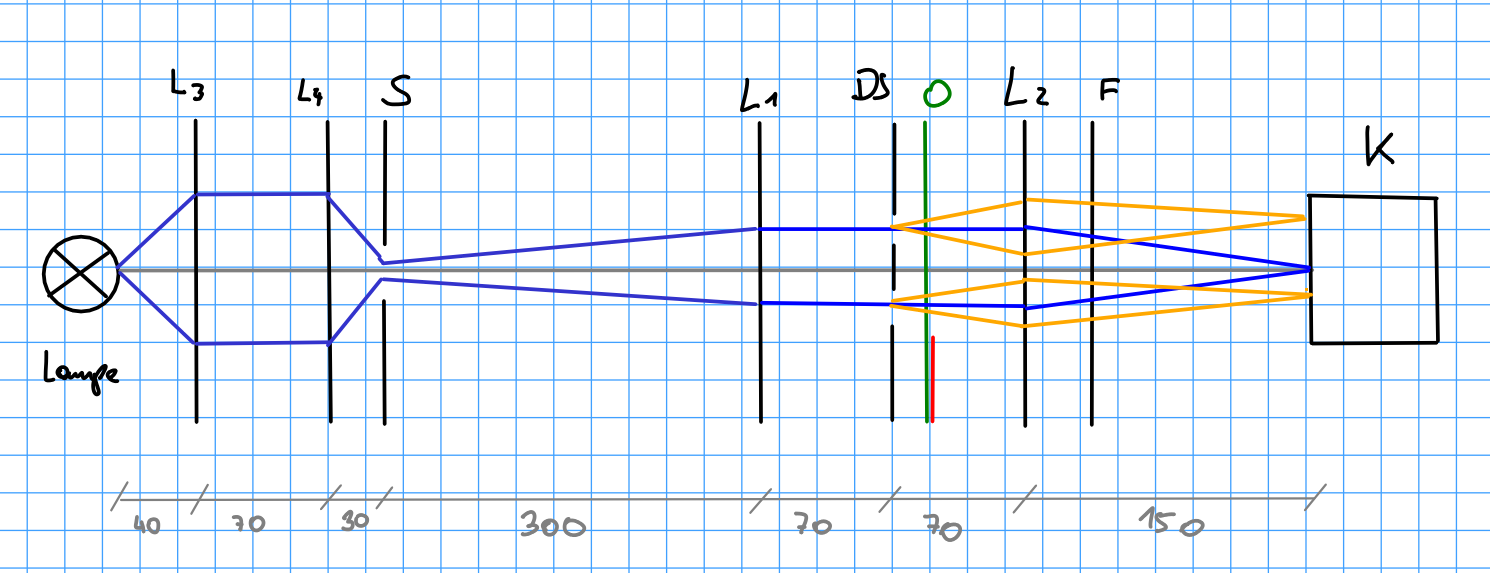
\includegraphics[scale=1]{strahlen.png}
\end{figure}

\newpage


\section{Versuchsdurchführung und Messwerte}

Die Versuchsergebnisse werden von der Kamera aufgenommen. Diese wird mit einem Computer und der Software \textit{IC Capture} gesteuert.


\subsection{Zusammenhang zwischen Größe der Lichtquelle und Interferenzmuster}

Bei einer großen Lichtquelle kann räumliche Kohärenz auftreten. Daraus resultiert ein schwächerer Konstrast. Die Größe der Lichtquelle wird durch die verstellbare Spaltblende realisiert. Für diesen Versuch wurde monochromatisches Licht verwendet. Dann wurde der $633~$nm Bandpassfilter in den Strahlengang gedreht und der  Doppelspalt mit $d_2 = 0.23~$mm in den Strahlengang geschoben.

Dann wurden 6 geeignete Größen der Lichtquelle gewählt, um den Verlauf des Kontrastes gemäß im Bereich $0 < 2\cdot w < 1.5 \cdot \lambda\cdot f_1 / d$ darstellen zu können. Dafür wurde zunächst die Spaltbreite des Kontrast-Minimums bestimmt. Beim Wert 0 der Mikrometerschraube war der Spalt jedoch noch nicht ganz geschlossen, sodass mit einer negativen Spaltbreite $A=(-0.23 \pm 0.06)$~mm begonnen wurde, um den Spalt auch ganz geschlossen zu halten. Die ersten Bilder wurden dann bei dem Ablesewert $A=0~$mm durchgeführt, sodass dieser unter Berücksichtigung des Offsets eigentlich bei $0.23~$mm ist.
Für die gewählten Größen der Lichtquelle wurde jeweils ein Foto des Beugungsmusters aufgenommen und zusätzlich werden die Grauwerte mit dem Programm ImageJ grafisch dargestellt.

Der Konstrast kann nun mit Formel~\ref{eq:kontrast} berechnet werden.

Die Aufnahmen der Interferenzmuster und die grafische Darstellung der Grauwerte sind im folgenden aufgelistet.

\begin{figure}[H]
\centering
\caption{Interferenzmuster für $2\cdot w \approx (0.23\pm0.06)~$mm}
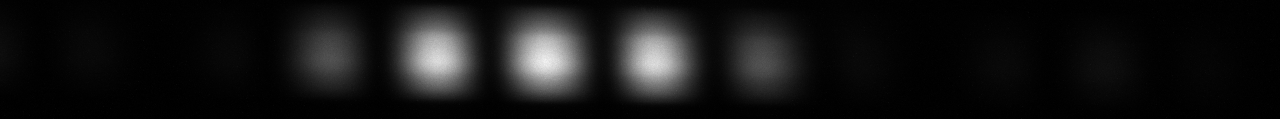
\includegraphics[width=9cm]{moodle/img2.png}
\end{figure}

\begin{figure}[H]
\centering
\caption{Grafische Darstellung der Intensitäten beim Interferenzmuster für $2\cdot w \approx (0.23\pm0.06)~$mm.}
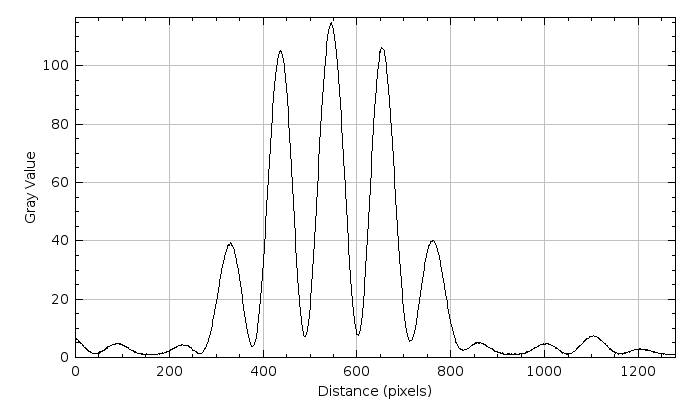
\includegraphics[width=9cm]{moodle/img2_graph.png}
\end{figure}



\begin{figure}[H]
\centering
\caption{Interferenzmuster für $2\cdot w \approx (0.48\pm0.06)~$mm}
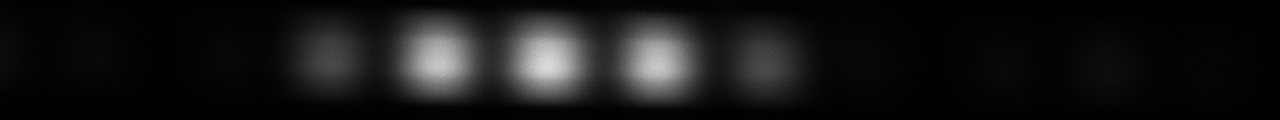
\includegraphics[width=9cm]{moodle/img3.png}
\end{figure}

\begin{figure}[H]
\centering
\caption{Grafische Darstellung der Intensitäten beim Interferenzmuster für $2\cdot w \approx (0.48\pm0.06)~$mm.}
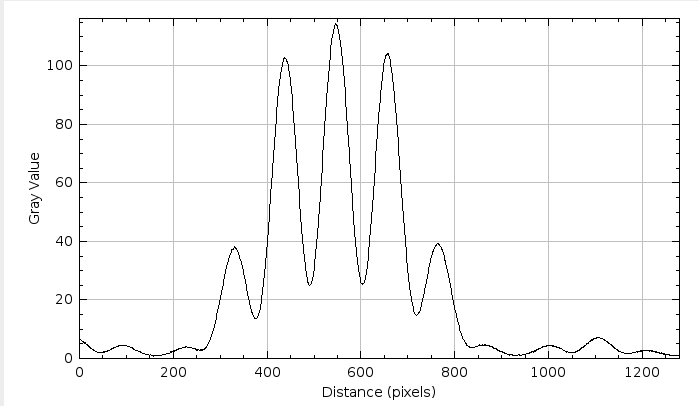
\includegraphics[width=9cm]{moodle/img3_graph.png}
\end{figure}



\begin{figure}[H]
\centering
\caption{Interferenzmuster für $2\cdot w \approx (0.73\pm0.06)~$mm}
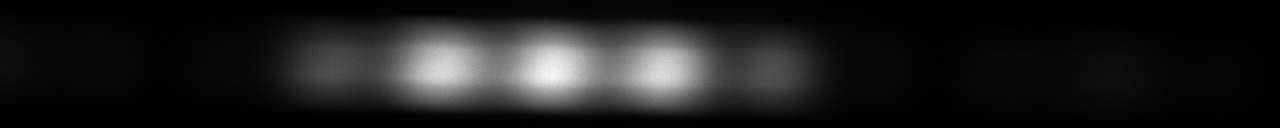
\includegraphics[width=9cm]{moodle/img4.png}
\end{figure}

\begin{figure}[H]
\centering
\caption{Grafische Darstellung der Intensitäten beim Interferenzmuster für $2\cdot w \approx (0.73\pm0.06)~$mm.}
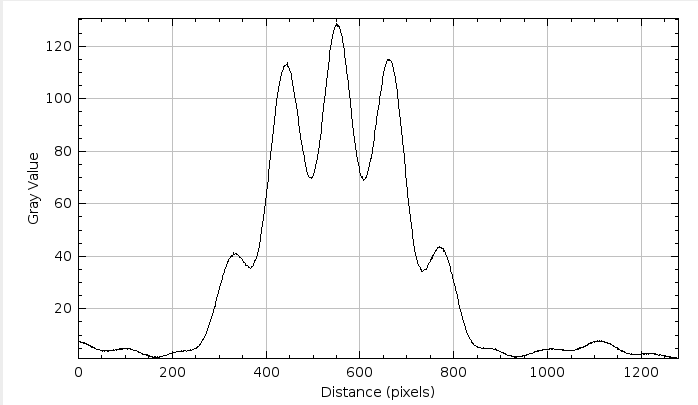
\includegraphics[width=9cm]{moodle/img4_graph.png}
\end{figure}




\begin{figure}[H]
\centering
\caption{Interferenzmuster für $2\cdot w \approx (0.97\pm0.06)~$mm}
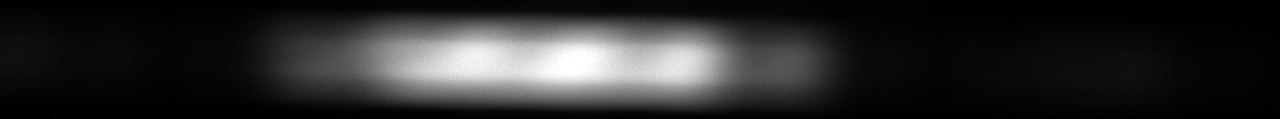
\includegraphics[width=9cm]{moodle/img5.png}
\end{figure}

\begin{figure}[H]
\centering
\caption{Grafische Darstellung der Intensitäten beim Interferenzmuster für $2\cdot w \approx (0.97\pm0.06)~$mm.}
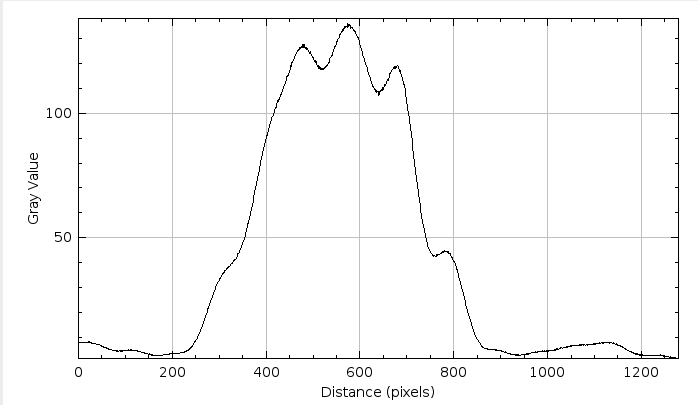
\includegraphics[width=9cm]{moodle/img5_graph.png}
\end{figure}



\begin{figure}[H]
\centering
\caption{Interferenzmuster für $2\cdot w \approx (1.23\pm0.06)~$mm}
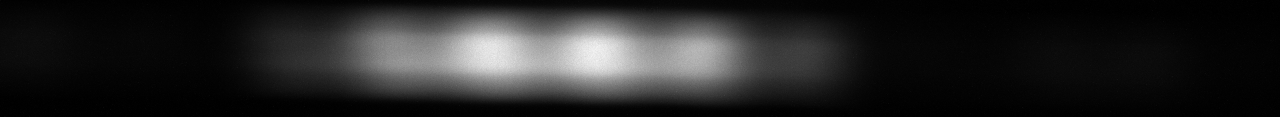
\includegraphics[width=9cm]{moodle/img6.png}
\end{figure}

\begin{figure}[H]
\centering
\caption{Grafische Darstellung der Intensitäten beim Interferenzmuster für $2\cdot w \approx (1.23\pm0.06)~$mm.}
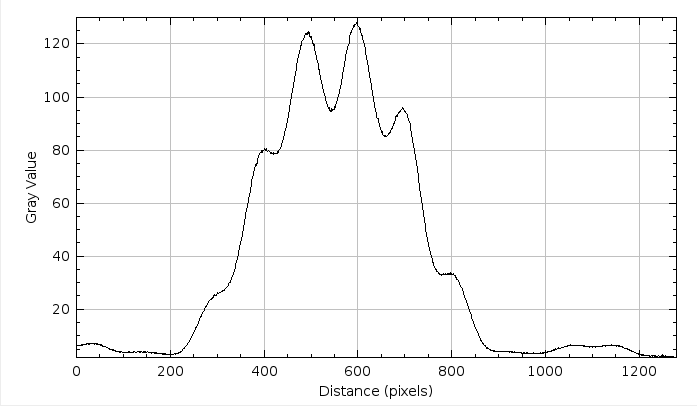
\includegraphics[width=9cm]{moodle/img6_graph.png}
\end{figure}





\begin{figure}[H]
\centering
\caption{Interferenzmuster für $2\cdot w \approx (1.45\pm0.06)~$mm}
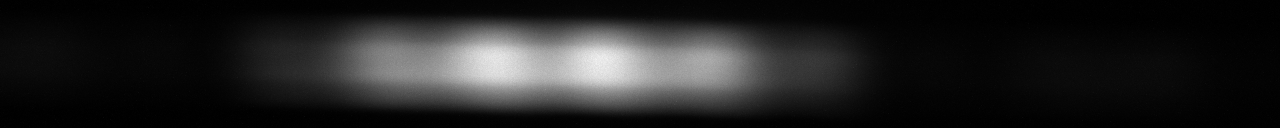
\includegraphics[width=9cm]{moodle/img7.png}
\end{figure}

\begin{figure}[H]
\centering
\caption{Grafische Darstellung der Intensitäten beim Interferenzmuster für $2\cdot w \approx (1.45\pm0.06)~$mm.}
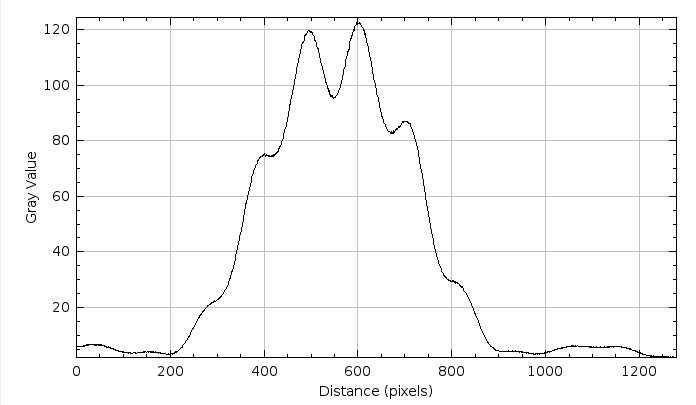
\includegraphics[width=9cm]{moodle/img7_graph.png}
\end{figure}



\begin{table}[H]
\caption{Beugungsextremum 0. Ordnung, bezeichnet als $I_0$, Beugungsextrema 1. Ordnung $I_{-1}$ links von $I_0$ und $I_{+1}$ rechts von $I_0$. Die 0. Ordnung ist bei den ersten Messungen ein Maximum, wird aber später zu Minimum wegen Nullstelle im Kontrast.}
\begin{tabular}{l|rrrr}
$2\cdot w$ / mm & $I_0$ & $I_{-1}$ & $I_{+1}$ & $\overline{I_{1}}$ \\
\hline
0.23 & 114.891 & 7.118 & 7.597 & 7.358 \\
0.48 & 114.552 & 24.817 & 25.261 & 25.039 \\
0.73 & 128.655 & 69.862 & 69.026 & 69.444 \\
0.97 & 135.926 & 117.512 & 107.198 & 112.355 \\
1.23 & 94.551 & 124.517 & 128.076 & 126.297 \\
1.45 & 95.355 &  119.835 & 122.570 & 121.202
\end{tabular}
\end{table}





%
%\begin{table}[H]
%\caption{Beugungsextremum 0. Ordnung, bezeichnet als $I_0$, Beugungsextrema 1. Ordnung $I_{-1}$ links von $I_0$ und $I_{+1}$ rechts von $I_0$. Die 0. Ordnung ist bei den ersten Messungen ein Maximum, wird aber später zu Minimum wegen Nullstelle im Kontrast.}
%\begin{tabular}{l|rrrr}
%Spaltbreite & $I_0$ & $I_{-1}$ & $I_{+1}$ & $\overline{I_{1}}$ \\
%\hline
% & 114.891 & 7.118 & 7.597 & 7.358 \\
% & 114.552 & 24.817 & 25.261 & 25.039 \\
% & 128.655 & 69.862 & 69.026 & 69.444 \\
% & 135.926 & 117.512 & 107.198 & 112.355 \\
% & 94.551 & 124.517 & 128.076 & 126.297 \\
% & 95.355 &  119.835 & 122.570 & 121.202
%\end{tabular}
%\end{table}


\newpage
\subsection{Zusammenhang zwischen spektraler Breite und Interferenzmuster}

Beim zweiten Versuch ist diesmal das Licht räumlich kohärent, dafür variiert die spektrale Breite (und damit die zeitliche Kohärenz). Die Theorie sagt, dass die 0. Beugungsordnung mit der höchsten Intensität dargestellt wird und die Intensität nach außen hin nachlässt. Es wurde die Spaltblende so eingestellt, dass das Licht mit 0.43 mm Spaltabstand räumlich gut kohärent ist. Danach wurde ein Beugungsbild mit dem 633 nm Bandpassfilter, mit dem Langpassfilter und ohne Filter aufgenommen. 

\begin{figure}[H]
\centering
\caption{Beugungsmuster mit Langpassfilter}
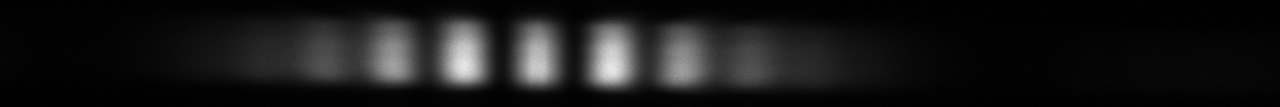
\includegraphics[width=9cm]{moodle/img_LP.png}
\end{figure}

\begin{figure}[H]
\centering
\caption{Beugungsmuster mit 633~nm-Bandpassfilter}
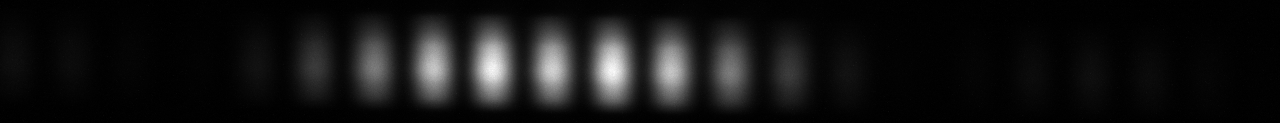
\includegraphics[width=9cm]{moodle/img_633BP.png}
\end{figure}

\begin{figure}[H]
\centering
\caption{Beugungsmuster ohne Filter}
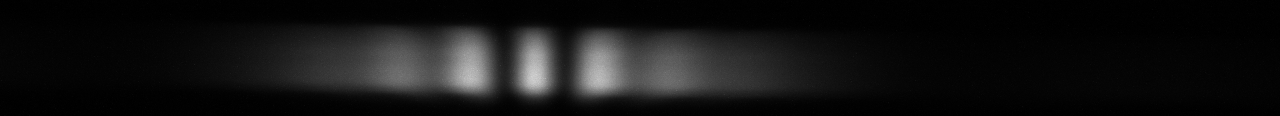
\includegraphics[width=9cm]{moodle/img__.png}
\end{figure}

\begin{figure}[H]
\centering
\caption{Transmissionsspektrum des Langpassfilters (blau) und des Bandpassfilters (orange). Quelle: \cite{quelle6}}
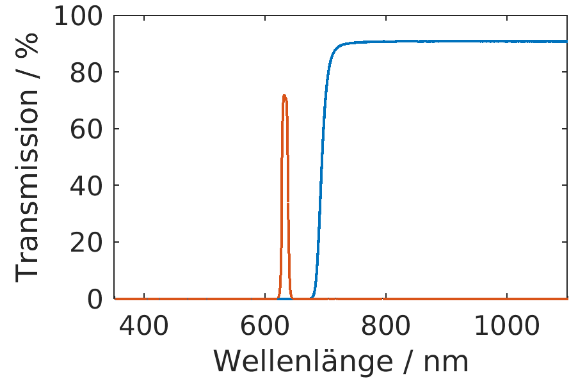
\includegraphics[width=5cm]{moodle/filter.png}
\end{figure}



\subsection{Bestimmung der Dicke der Polyacrylat-Schicht anhand des Interferenzmusters}

Hier wurde der vorderste Doppelspalt mit 0.43 mm Spaltabstand verwendet und alle Filter aus dem Strahlengang gedreht. Danach wurde die mit Polyacrylat überzogene Probe in den Strahlengang eingebracht und mit einer Justierschraube verschoben, sodass die Polyacrylat-Schicht nur einen der beiden Spalte abdeckt. Dann wurde das Bild des verschobenen und ein Bild des nicht verschobenen Beugungsmusters, sowie ein Bild ohne Polyacrylat als Referenzwert aufgenommen.

\begin{figure}[H]
\centering
\caption{Darstellung des Beugungsmusters mit und ohne Verschiebung}
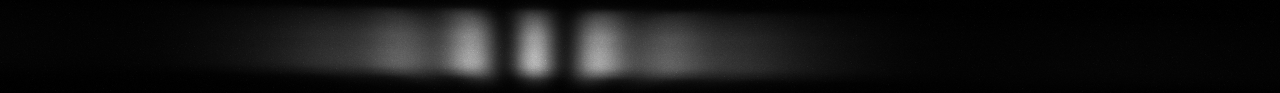
\includegraphics[width=9cm]{moodle/img_noShift.png}
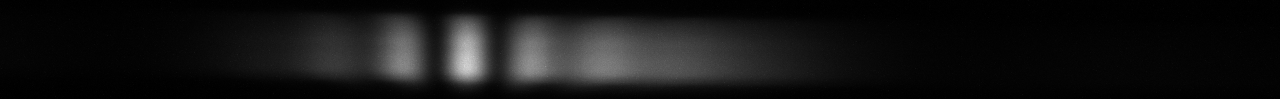
\includegraphics[width=9cm]{moodle/img_Shift.png}
\end{figure}


\subsection{Maximale Größe des Lichts für räumliche Kohärenz}

In diesem Versuch wurde wieder monochromatisches Licht mit einem Bandpass von 633 nm verwendet. Für drei Doppelspalten ($d_1=0.43~$mm, $d_2=0.23$~mm und $d_3=0.13$~mm) wird die Blende so reguliert, dass der Kontrast gerade verschwindet. Die Werte werden an der $\mu$m-Schraube abgelesen.

\begin{table}[H]
\caption{Ablesewerte der Mikrometerschraube. $x_1$ sind die Werte für den Spalte mit $d_1=0.43$~mm, $x_2$ für den Spalte mit $d_2=0.23$~mm und $x_3$ für den Spalt mit $d_3=0.13~$mm. Berechnung des Mittelwertes und der Standardabweichung.}
\begin{tabular}{c|rrr}
Messung & $x_1$ / mm & $x_2$ / mm & $x_3$ / mm \\
\hline
1 & 0.325 & 0.695 & 1.740 \\
2 & 0.315 & 0.722 & 1.865 \\
3 & 0.322 & 0.715 & 1.900 \\
4 & 0.318 & 0.725 & 1.655 \\
\hline 
$\overline{x_i}$ & 0.320 & 0.714 & 1.790 \\
$\sigma_i$ & 0.004 & 0.014 & 0.113
\end{tabular}

\end{table}


\newpage



\section{Auswertung}



\subsection{Zusammenhang zwischen Größe der Lichtquelle und Interferenzmuster}

Gleichung~\eqref{eq:kontrast} berechnet den Kontrast. Zusätzlich betrachten wir den Betrag des Kontrasts, da wir in der Messreihe eine Nullstelle des Kontrasts haben. Mit Fehlerrechnung ergibt sich
\begin{align*}
K = \left|\frac{I_\text{0,max}-I_\text{1,min}}{I_\text{0,max}+I_\text{1,min}} \right| \pm \left| \frac{ 2\cdot I_{1,\text{min}} \cdot \Delta I_{0,\text{max}} }{(I_\text{0,max}+I_\text{1,\text{min}})^2}  + \frac{ 2\cdot I_{0,\text{max}} \cdot \Delta I_{1,\text{min}} }{(I_\text{0,max}+I_\text{1,min})^2} \right|
\end{align*}



\begin{table}[H]
\caption{Berechnung des Kontrasts, Beugungsextremum 0. Ordnung $I_0$, mittleres Beugungsextremum 1. Ordnung $I_1$.}
\begin{tabular}{l|rr|r}
$2\cdot w$ / mm & $I_0$ & $I_1$ & $K$ \\
\hline
0.23 & 114.891 &   7.358 & $0.880$ \\
0.48 & 114.552 &  25.039 & $0.641$ \\
0.73 & 128.655 &  69.444 & $0.299$ \\
0.97 & 135.926 & 112.355 & $0.095$ \\
1.23 & 94.551  & 126.297 & $0.144$ \\
1.45 & 95.355 &  121.202 & $0.119$
\end{tabular}
\end{table}

Man kann nun den gemessenen Kontrast mit dem theoretischen Kontrast vergleichen. Dazu zeichnet die Kurve des theoretischen Kontrasts gemäß Gleichung~\eqref{eq:kontrast}.

\begin{figure}[H]
\centering
\caption{Kontrast abhängig von der Größe der Lichtquelle. Die blaue Linie ist der theoretische Kontrastverlauf abhängig von der Öffnung der Spaltblende. Die roten Punkte sind die gemessenen Kontraste.}
\label{fig:curve_task1}
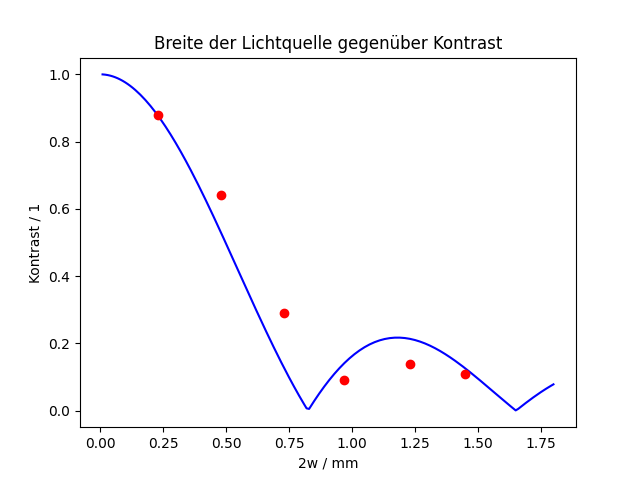
\includegraphics[width=12cm]{curve_task1.png}
\end{figure}




\subsection{Zusammenhang zwischen spektraler Breite und Interferenzmuster}

Da das Beugungsbild beim Interferenzmuster ohne Filter nach außen hin unscharf wird, wird auch der Kontrast geringer. Das sieht man in Grafik~\ref{fig:filter_kurven}. Zusätzlich sieht man, dass der Bandpass-Filter am wenigsten Frequenz durchlässt. Hier ist der Kontrast auch weiter außen noch größer. Grafisch erkennt man es, dass das Interferenzmuster beim Bandpass-Filter nach außen hin am wenigsten verschwommen ist.

\begin{figure}[H]
\centering
\caption{Darstellung der Intensitäten der Beugungsmaxima abhängig vom Filter.}
\label{fig:filter_kurven}
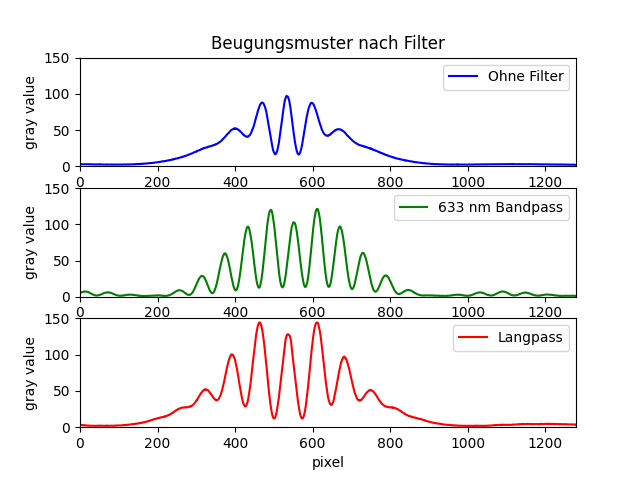
\includegraphics[width=12cm]{filter.png}
\end{figure}



\subsection{Bestimmung der Dicke der Polyacrylat-Schicht anhand des Interferenzmusters}

Es werden die beiden 0. Ordnungen verglichen. Ohne Polyacrylatschicht ist das gesuchte Maximum bei Pixel 534, während es ohne Polyacrylatschicht bei 467 ist. Als Unsicherheit werden 2 Pixel angenommen, da die unmittelbar benachbarten Grauwerte relativ ähnlich sind. Als Verschiebung ergibt sich
\begin{align*}
x_{\delta} = (67 \pm 4)~\text{pixel}
\end{align*}

\begin{figure}[H]
\centering
\caption{Darstellung des Beugungsmusters mit und ohne Verschiebung}
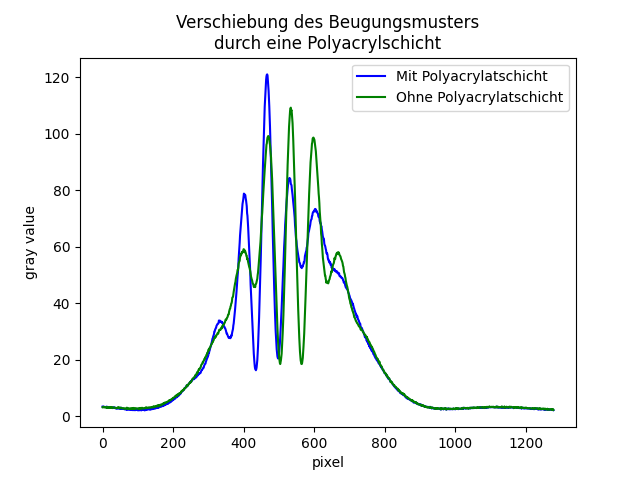
\includegraphics[width=9cm]{shift_noshift.png}
\end{figure}


Es muss nun die Anzahl der Pixel in $\mu$m umgerechnet werden. Hierfür wird die Formel~\eqref{eq:umrechnung} verwendet. Dafür wird zuerst die Distanz zwischen dem $0$-tem und dem $4$-ten Maximum benötigt. Wir verwenden als Referenz zur Bestimmung der $\mu$ pro Pixel das Interferenzmuster mit dem Bandpass-Filter aus Aufgabe 2, dafür die Formel ein konstantes $\lambda$ gebraucht wird. Die beiden Maxima sind in Grafik~\ref{fig:633nm_task3} dargestellt.

\begin{figure}[H]
\centering
\caption{Beugungsmuster des 633 nm Bandpassfilters, wobei das 0. und das 4. Maximum eingezeichnet sind. (rote Kreuze)}
\label{fig:633nm_task3}
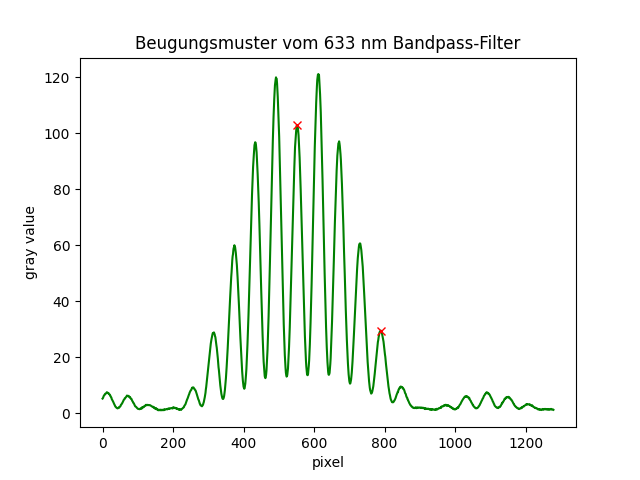
\includegraphics[scale=1]{633_for_task3.png}
\end{figure}

Aus Grafik~\ref{fig:633nm_task3} ergibt sich
\begin{align*}
|x_0-x_4| = (238 \pm 4)~\text{pixel}
\end{align*}
Der Umrechnungsfaktor zwischen Pixel und $\mu$m ergibt sich nun aus Formel~\eqref{eq:umrechnung}.
\begin{align*}
Z = \frac{f\cdot \tan\left(\operatorname{arcsin}\left(\frac{4\cdot \lambda}{d}\right)\right)}{|x_0-x_4|}
\end{align*}
wobei $f=150~$mm die Brennweite der Linse, $\lambda=633~$nm die Frequenz des Lichtes und $d=0.43~$mm der Spaltabstand ist (s. Versuch 2). Insgesamt ergibt sich inkl. Fehlerrechnung
\begin{align}
Z = (3.71 \pm 0.24)~\mu\text{m} / \text{pixel}
\end{align}

Mit der Umrechnung kann man jetzt $b=x_\delta\cdot Z$ berechnen. Damit hat man die Verschiebung $b$ in $\mu$m. Diese
\begin{align*}
b = (248.65\pm23.65)~\mu\text{m}
\end{align*}
Durch die Formel~\eqref{eq:theta} kann man nun den Winkel $\theta$ berechnen. Diesen in Formel~\eqref{eq:schichtdicke} eingesetzt ergibt dann insgesamt
\begin{align*}
t = (1.45\pm0.11)~\mu\text{m}
\end{align*}



\subsection{Maximale Größe des Lichts für räumliche Kohärenz}


Aus der bekannten Beziehung $2\cdot w \le \lambda\cdot f_1 /d$ ergibt sich inkl. Fehlerrechung
\begin{align*}
2\cdot w = \frac{\Delta f_1 \cdot d \cdot \lambda + f_1\cdot\lambda\cdot \Delta d + f_1\cdot d\cdot \Delta \lambda }{d^2}
\end{align*}
Aus $\le$ wird Gleichheitszeichen, da ein Maximum für $2\cdot w$ gesucht wird.


Durch Einsetzen erhält man
\begin{table}[H]
\caption{Größe des Lichts ($2\cdot w$) bei gegebenem Doppelspaltabstand $d_i$. Zusätzlich die gemessenen Werte $x_i$.}
\label{tab:task4}
\begin{tabular}{r|rr}
$d_i$ / mm & $2\cdot w$ / $\mu$m & $x_i$ / $\mu$m \\
\hline
0.43 & $441 \pm 15$ & 320 \\
0.23 & $825 \pm 36$ & 714\\
0.13 & $1460 \pm 89$ & 1790
\end{tabular}

\end{table}


\begin{figure}[H]
\centering
\caption{Maximale Größe des Lichts ($2\cdot w$) abhängig vom Doppelspaltabstand $d$.}
\label{fig:task4}
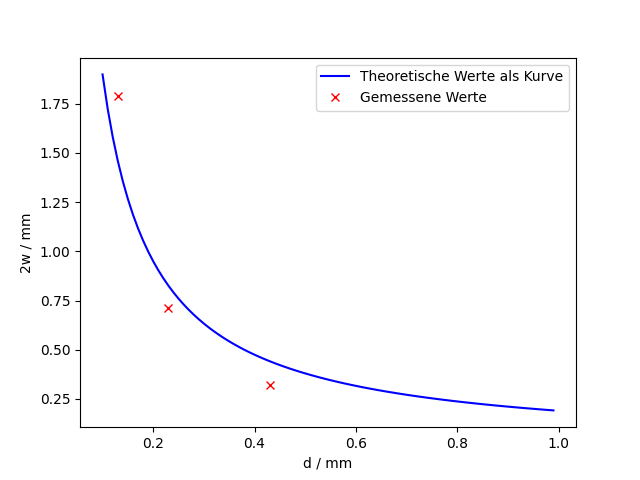
\includegraphics[scale=0.7]{task4.png}
\end{figure}

Als Unsicherheiten verwenden wir hier $\Delta\lambda=10~$nm, $\Delta f_1 = 2$~mm, $\Delta d_i = 0.005~$mm.

\newpage
\section{Diskussion und Zusammenfassung}

\subsection{Zusammenhang zwischen Größe der Lichtquelle und Interferenzmuster}

Man sieht deutlich, dass der Kontrast zuerst mit Größe des Spaltes abnimmt. Nach einem Minimum steigt der Kontrast wieder. Der Kontrast selbst ist immer positiv, ändert sich aber mit der Größe der Lichtquelle. Der grafische Zusammenhang wird in Grafik~\ref{fig:curve_task1} veranschaulicht. Im wesentlichen bestätigen die Experimente die durch die Vorbereitung gelernten Inhalte. Die Grundlage dieses Versuchs ist Grafik~\ref{fig:versuch1_grundlagen}.


\begin{figure}[H]
\caption{Theoretischer Hintergrund zu diesem Versuch: mehrere Wellen gleicher Wellenlänge (und unterschiedlicher Phasenverschiebung) überlagert lassen den Kontrast gleichmäßig abnehmen. Quelle: \cite{quelle6}.}
\label{fig:versuch1_grundlagen}
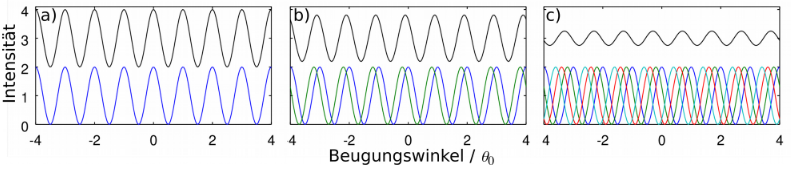
\includegraphics[width=10cm]{diskussion2.png}
\end{figure}




\subsection{Zusammenhang zwischen spektraler Breite und Interferenzmuster}


Dieser Versuch zeigt, dass bei verschiedenen Frequenzen der Kontrast des Beugungsbildes nach außen hin abnimmt, während bei einheitlicher Wellenlänge der Kontrast nach außen hin erhalten bleibt. Dies deckt sich mit der Theorie aus~\cite{quelle6}. Wie zu erwarten war hat das Beugungsbild beim Bandpass-Filter den höchsten Kontrast. Durch die einheitliche Wellenlänge wird der Kontrast nach außen nicht kleiner. Dieser Versuch veranschaulicht Grafik~\ref{fig:versuch2_grundlagen}.

\begin{figure}[H]
\caption{Theoretischer Hintergrund zu diesem Versuch: mehrere Wellen unterschiedlicher Wellenlänge überlagert lassen den Kontrast nach außen hin abnehmen. Quelle: \cite{quelle6}.}
\label{fig:versuch2_grundlagen}
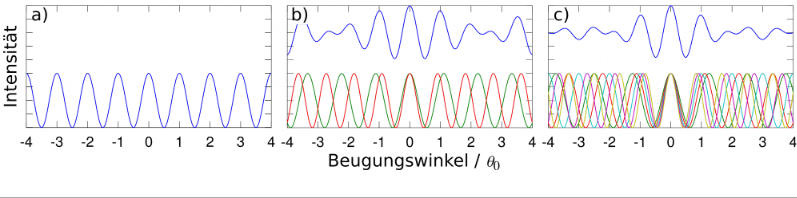
\includegraphics[width=10cm]{diskussion1.png}
\end{figure}




\subsection{Bestimmung der Dicke der Polyacrylat-Schicht anhand des Interferenzmusters}

Die Schichtdicke wurde bestimmt, indem man zuerst die Verschiebung eines charakteristischen Punktes (z.B.: Maximum 0. Ordnung) misst. Diese Verschiebung betrug im Versuch 67 Pixel. Danach wurde der Abstand zwischen 0. und 4. Begungsmaximum rechnerisch in $\mu$m bestimmt und aus der entsprechenden Grafik auch in Pixel abgelesen. Durch Verhältnisbildung konnte man die Verschiebung $b$ in $\mu$m feststellen. Daraus folgte durch trigonometrische Überlegung der Beugungswinkel $\theta$, aus dem dann die Schichtdicke berechnet werden konnte.

Bei den Berechnungen kamen einige trigonometrische Funktionen vor. Durch algebraische Vereinfachung konnte man teilweise auch die direkte Berechnung von Winkeln vermeiden, um die Genauigkeit zu steigern. Beispielhaft ist das an folgender Formel veranschaulicht.
\begin{align*}
b = f\cdot \tan\left(\operatorname{arcsin}\left(\frac{m\cdot \lambda}{d}\right)\right) = f\cdot \frac{m\cdot \lambda}{\sqrt{d^2 - m^2\cdot \lambda^2}}
\end{align*}


Die berechnete Schichtdicke ist
\begin{align*}
t = (1.45\pm0.11)~\mu\text{m}
\end{align*}



\subsection{Maximale Größe des Lichts für räumliche Kohärenz}

Grafik~\ref{fig:task4} zeigt den Verlauf der Kurve mit den theoretischen Werten für die maximale Größe der Lichtquelle. Da wir nur Werte für 3 verschiedene Doppelspalten haben, ist es nicht möglich einen statistischen Zusammenhang zu bestimmen. Allerdings scheint dieser optisch erkennbar zu sein.

Durch die Wahl der Unsicherheiten liegen die Messwerte außerhalb der theoretischen Kurve. Es wäre zu diskutieren, ob die Unsicherheiten zu streng gewählt wurden und dass man unter anderen Annahmen eine Übereinstimmung sehen würden.



%\newpage 
%\appendix
%\section{Python Skript}



\definecolor{commentgreen}{RGB}{2,112,10}
\definecolor{eminence}{RGB}{108,48,130}
\definecolor{weborange}{RGB}{255,165,0}
\definecolor{frenchplum}{RGB}{129,20,83}

\lstdefinelanguage{python}{
    morekeywords={def, for, range, abs, return},
    otherkeywords={<-,->, |>, \%\{, \}, \{, \, (, )},
    sensitive=true,
    morecomment=[l]{\#},
    morecomment=[n]{/*}{*/},
    morecomment=[s][\color{purple}]{:}{\ },
    morestring=[s][\color{orange}]"",
    commentstyle=\color{commentgreen},
    keywordstyle=\color{eminence},
    stringstyle=\color{red},
	basicstyle=\ttfamily,
	breaklines,
	showstringspaces=false,
	frame=tb
}
%\lstinputlisting[language=Python,captionpos=b, label=lst:test,caption={Python Skript}]{generate_numbers.py}

%\lstinputlisting[language=Python,captionpos=b, label=lst:test,caption={Bessel Auswertung}]{generate_numbers_bessel.py}


%\lstinputlisting[language=Python,captionpos=b, label=lst:test,caption={Zerstreuungslinse Auswertung}]{generate_numbers_zerstreuungslinse.py}


\newpage

\begin{thebibliography}{9}
\bibitem{quelle1} \url{https://www.youtube.com/watch?v=oFJCEGcwUiQ}, 07.11.2020, 00:15 Uhr
\bibitem{quelle2} \url{https://www.spektrum.de/lexikon/physik/abbesche-theorie/13}, 07.11.2020, 00:17 Uhr
\bibitem{quelle3} \url{https://www.univie.ac.at/mikroskopie/1_grundlagen/optik/opt_instrumente/7_abbe.htm}, 07.11.2020, 00:24 Uhr
\bibitem{quelle4} \url{https://physik.cosmos-indirekt.de/Physik-Schule/Rayleigh-Kriterium}, 07.11.2020, 00:26 Uhr
\bibitem{quelle5} \url{https://www.youtube.com/watch?v=PZaUY45ce8k}, 07.11.2020, 00:27 Uhr
\bibitem{quelle6} Unterlagen aus Moodle, H. Ditlbacher, bereitgestellt von der KF Universität Graz
\end{thebibliography}


\end{document}
